\section{Experiments}\label{sec:experiment}
\begin{table*}[!t]\label{tbl:comparison}
\centering
\begin{minipage}{\textwidth}
\centering
\resizebox{\textwidth}{!}{%
\renewcommand{\arraystretch}{1.2}
\begin{tabular}{|c|c||c|c||c|c|}
\hline 
 \multirow{ 2}{*}{\bf Dataset} & \multirow{ 2}{*}{\bf Balance} & \multicolumn{2}{c||} {\bf Fairlet Decomposition Cost}   & \multicolumn{2}{c|}{{\bf Fair Clustering Cost} ($k=20$)} \\
 \cline{3-6}
 &	& \citep{chierichetti2017fair} &  {\bf Ours} & \citep{chierichetti2017fair} &  {\bf Ours} \\
\hline
Diabetes (1000 points) & $0.8$\footnote{In~\citep{chierichetti2017fair}, based on the description of the experiment setup, the desired balance in all three datasets (including Diabetes) are 0.5. However, for Diabetes dataset, they have achieved the higher balance of value 0.8.} & $\sim9836$ & $2971$ & $\sim 9909$& 4149\\ 
\hline
 Bank (1000 points) & $0.5$ & $\sim5.46 \times 10^5$ & $5.24 \times 10^5$  & $\sim5.55\times 10^5$ & $6.03\times 10^5$\\
\hline
 Census (600 points) & $0.5$ & $\sim3.59 \times 10^7$ & $2.31\times 10^7$ & $\sim3.65 \times 10^7$ & $2.41\times 10^7$\\
 \hline
\end{tabular}
%dimension: 2, 3, 6
}
\caption{The table compares the performance of our fairlet-decomposition algorithm and the algorithm of~\citep{chierichetti2017fair}. We remark that the number for~\citep{chierichetti2017fair} mentioned in this table are not explicitly stated in their paper and we have extracted them from Figure 3 in their paper. Note that the cost denotes the total distances of the points to their fairlet/cluster centroids.}
\label{table:results}
\end{minipage}
\end{table*}

\iffalse
\begin{figure*}[!b]
\minipage{0.33\textwidth}
  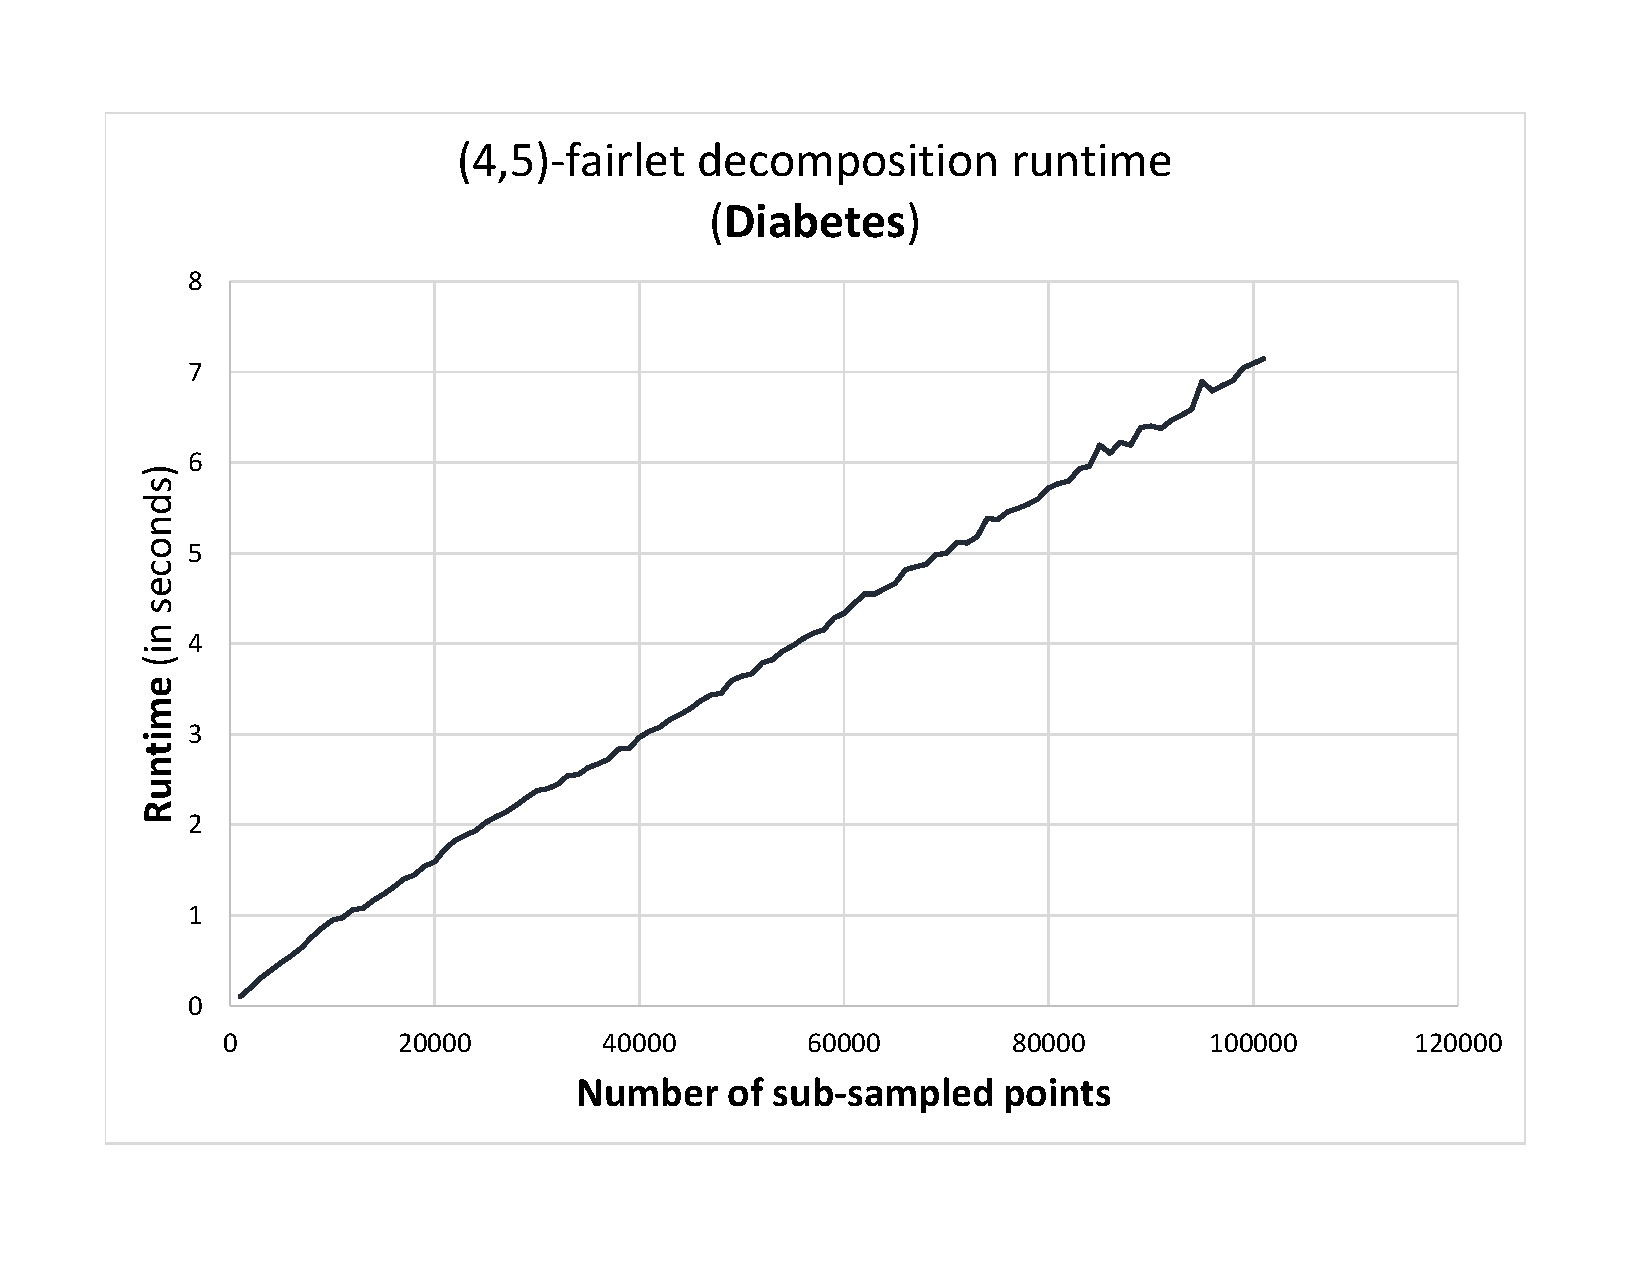
\includegraphics[width=1.1\linewidth]{uci-1-runtime.pdf}
  %\label{fig:diabetes}
\endminipage\hfill
\minipage{0.33\textwidth}
  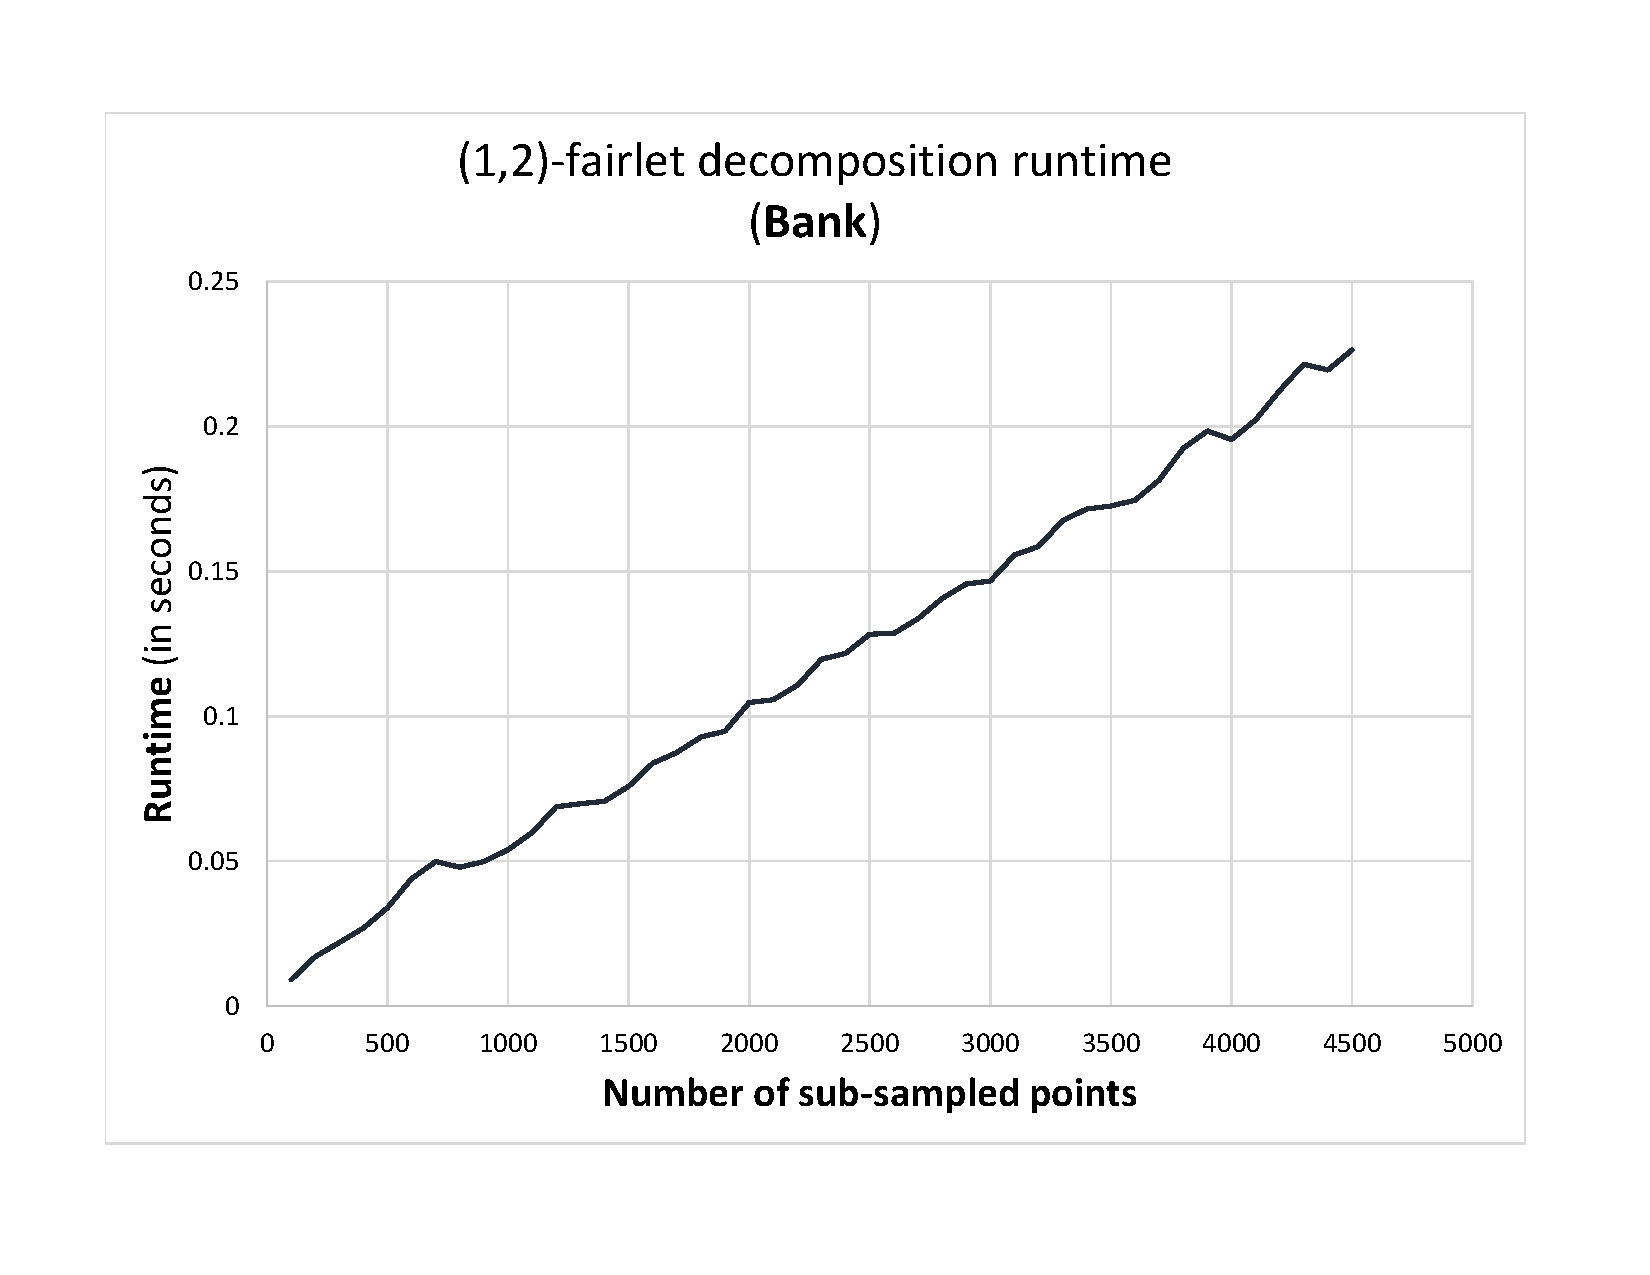
\includegraphics[width=1.1\linewidth]{uci-2-runtime.pdf}
  %\label{fig:bank}
\endminipage\hfill
\minipage{0.33\textwidth}%
  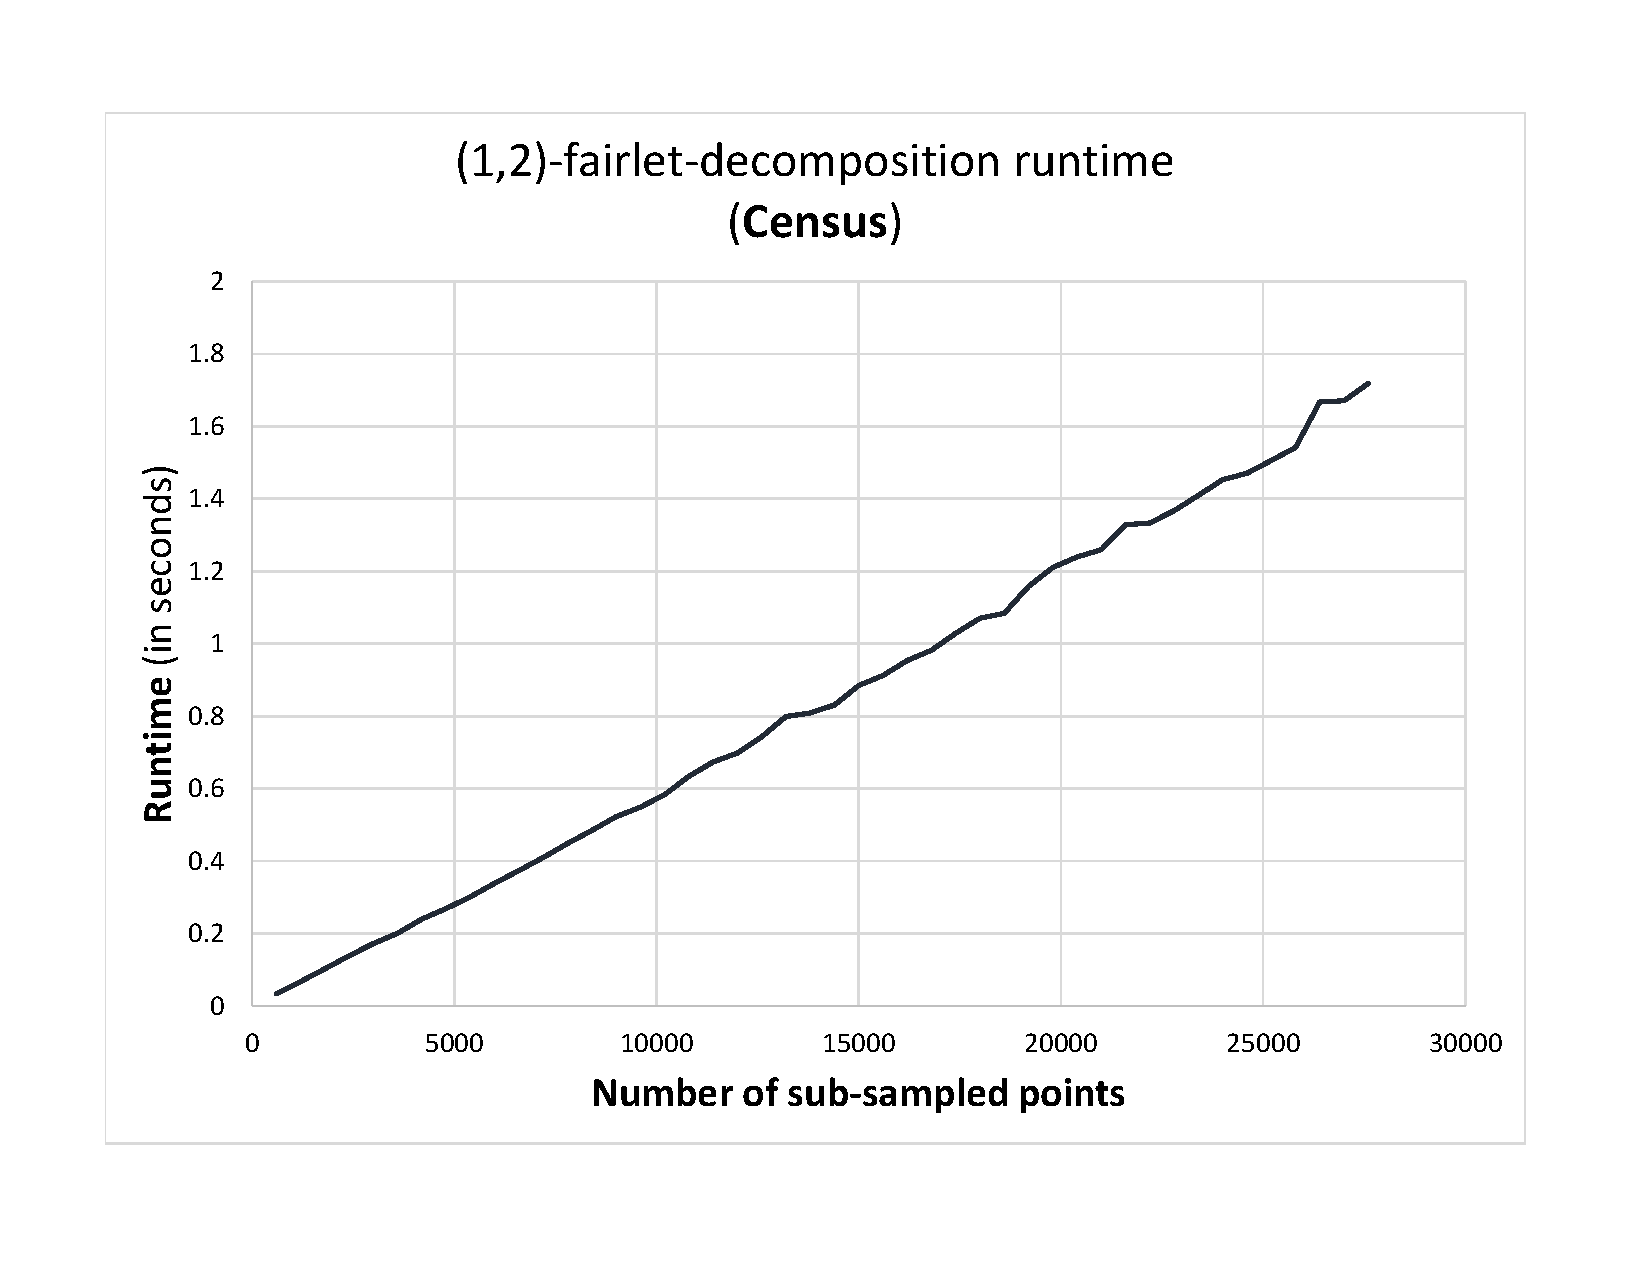
\includegraphics[width=1.1\linewidth]{uci-3-runtime.pdf}
  %\label{fig:census}
\endminipage
\caption{Each figure captures the running time of our fairlet decomposition algorithms with the specified balance parameter
on different number of sample points from one of the three datasets: Diabetes, Bank and Census.}\label{fig:runtime}
\end{figure*}
\fi
\begin{figure*}[!h]
\centering
\subfigure{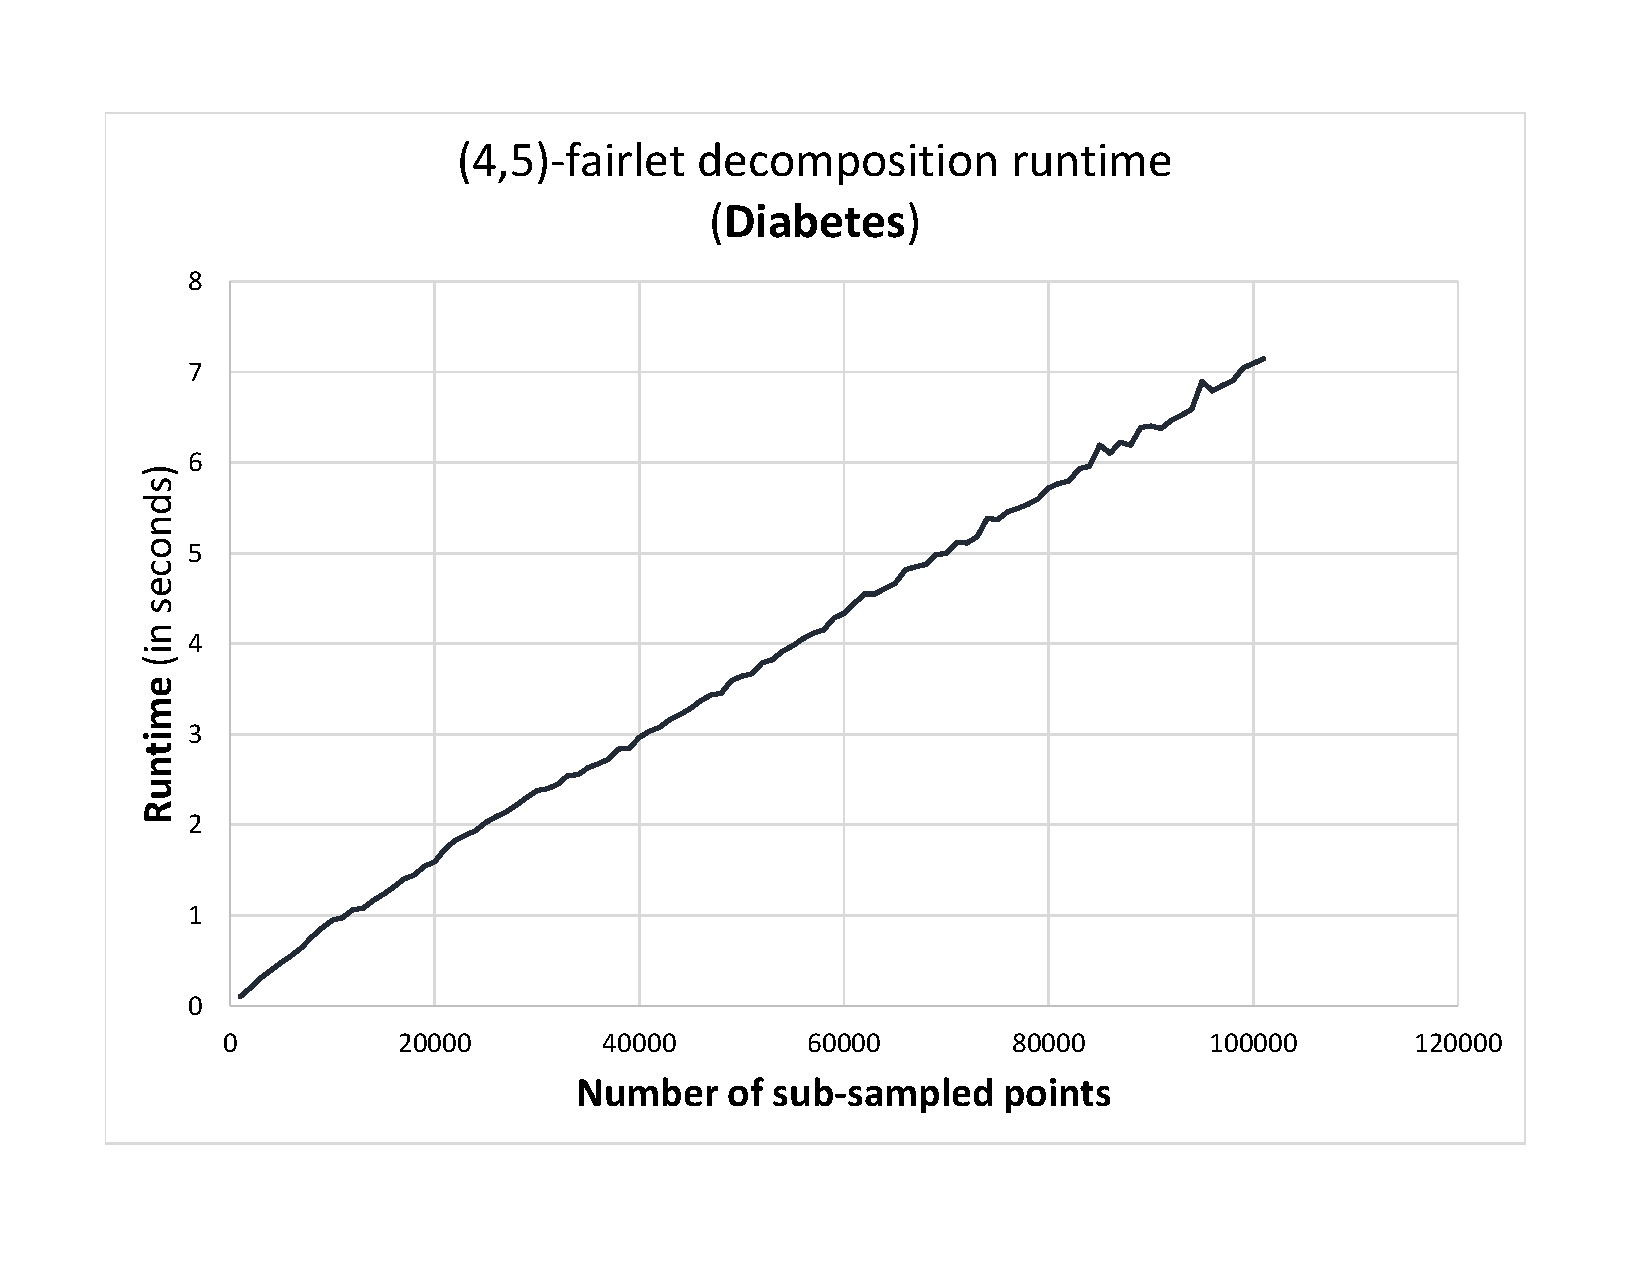
\includegraphics[width=0.49\textwidth]{uci-1-runtime.pdf}}
\subfigure{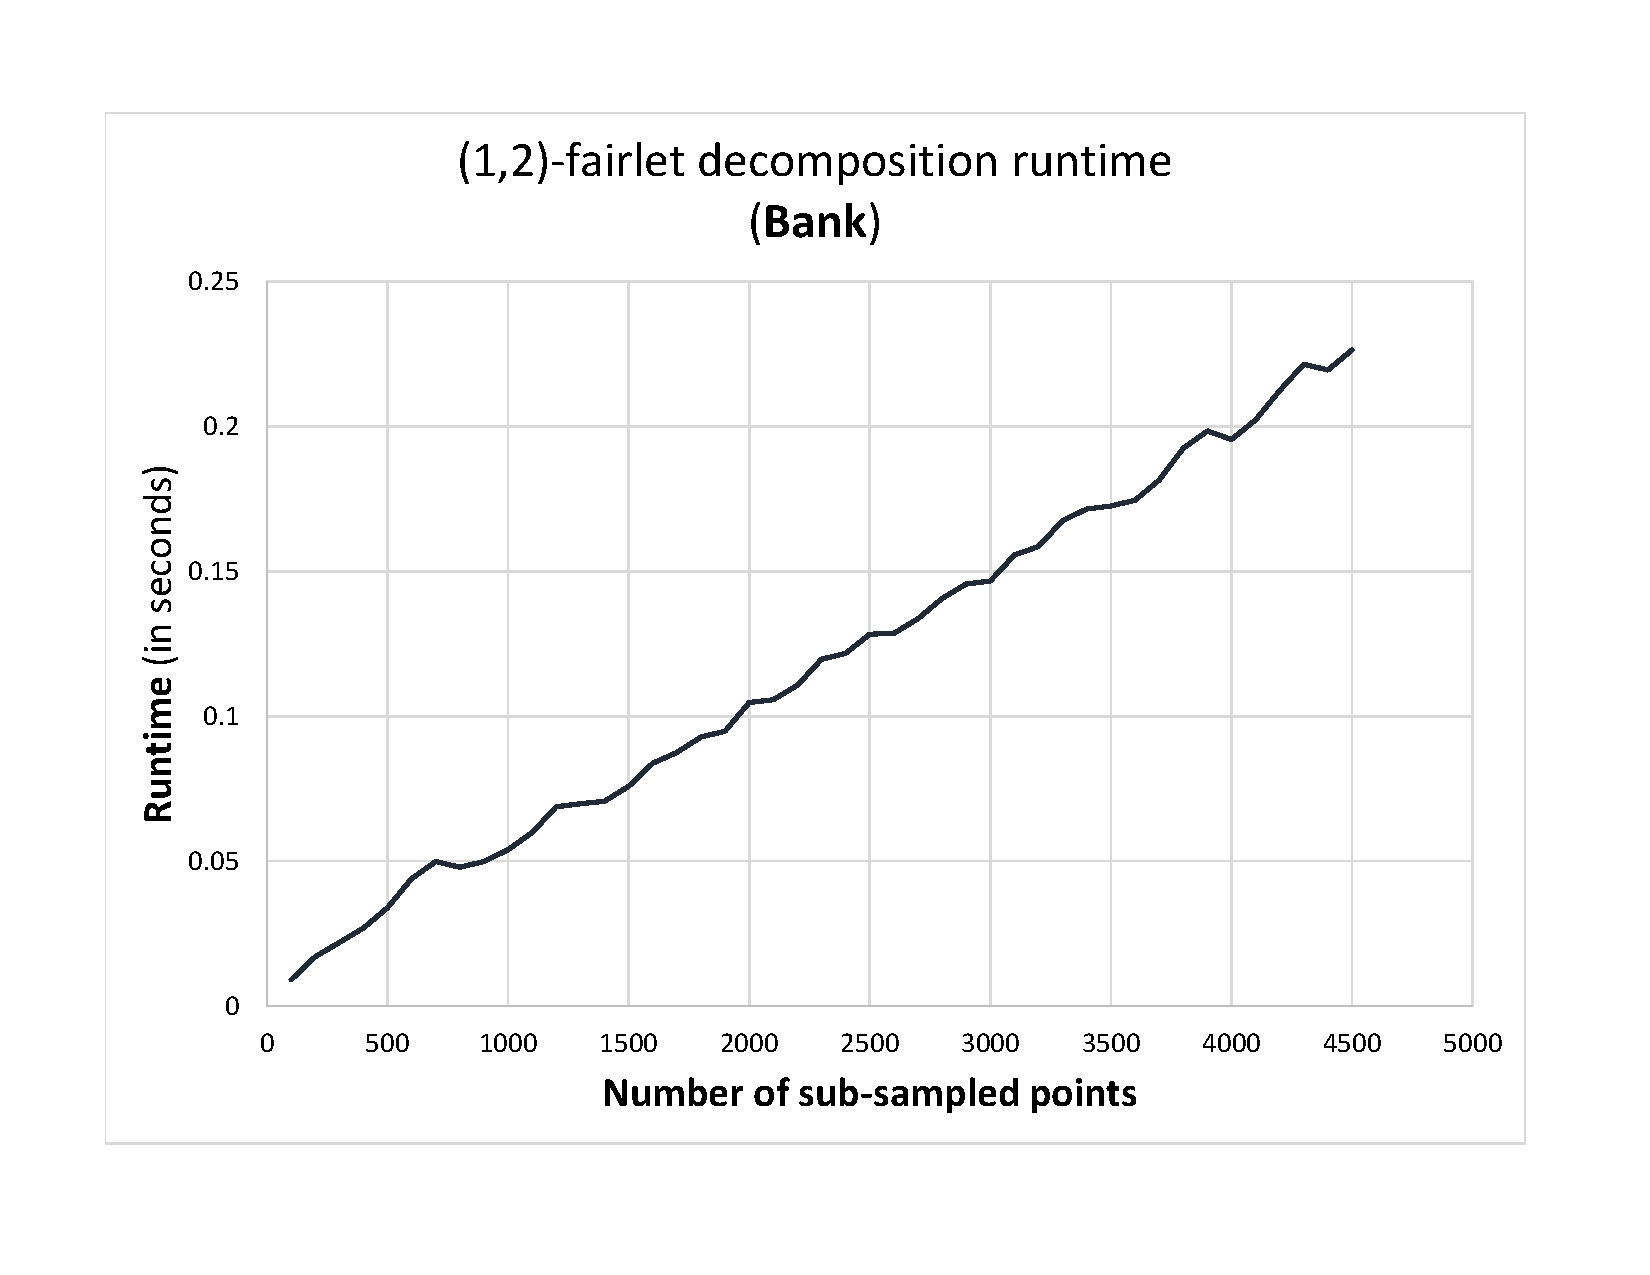
\includegraphics[width=0.49\textwidth]{uci-2-runtime.pdf}}
\centering
\subfigure{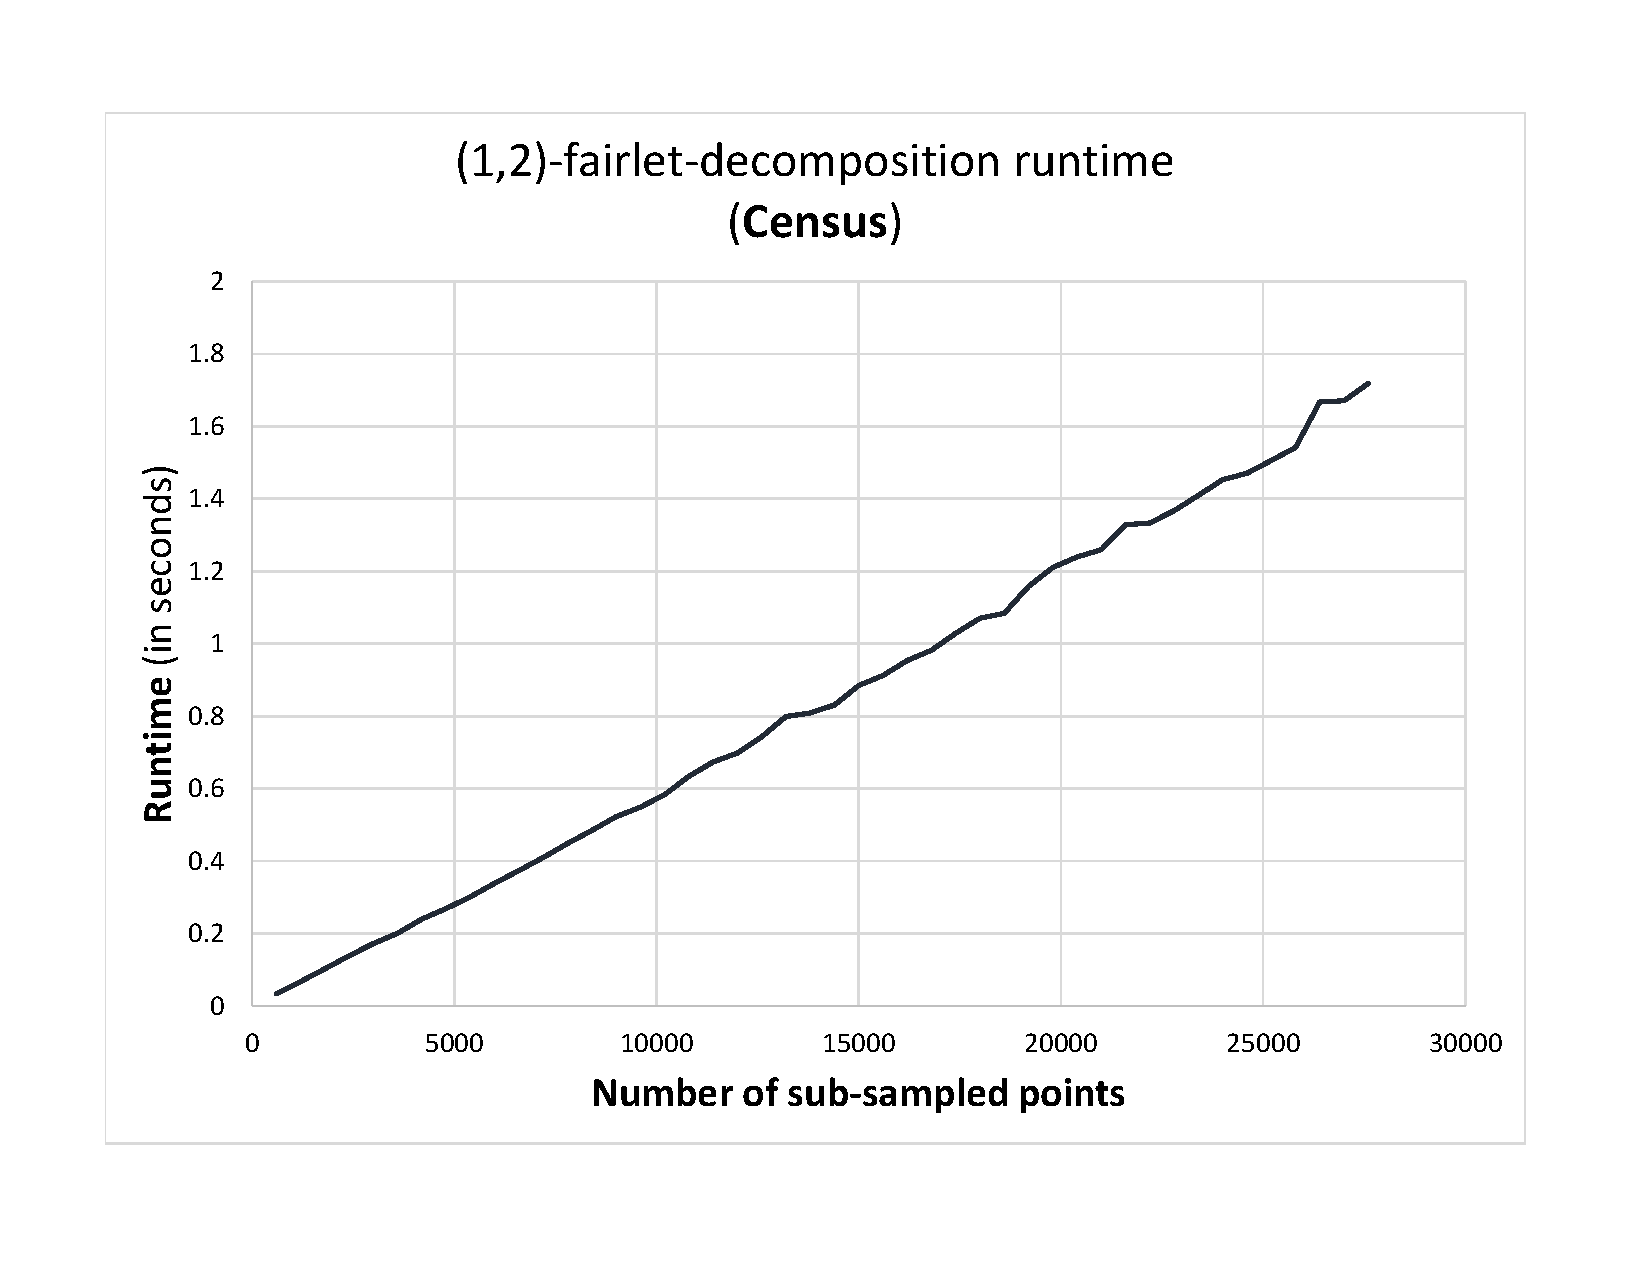
\includegraphics[width=0.49\textwidth]{uci-3-runtime.pdf}}
\subfigure{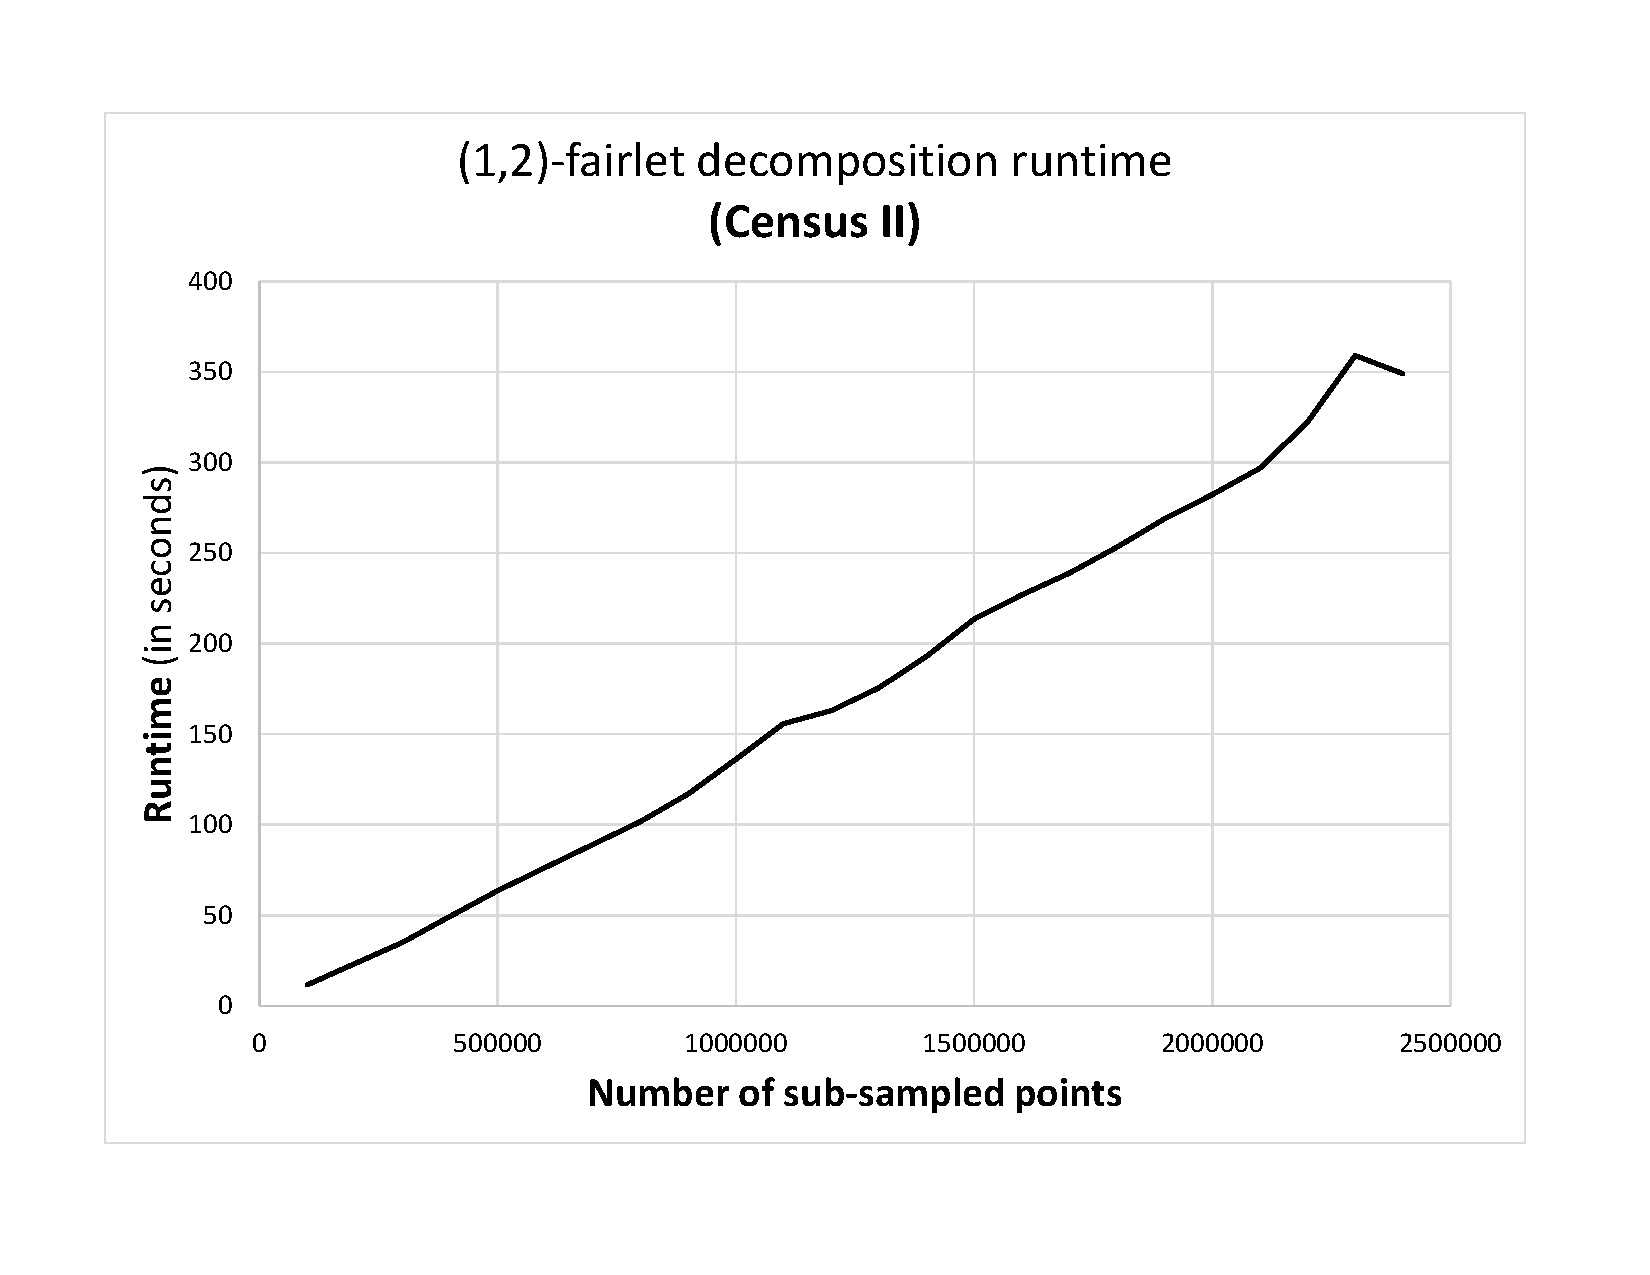
\includegraphics[width=0.49\textwidth]{uci-4-runtime.pdf}}
\caption{Each figure captures the running time of our fairlet decomposition algorithms with the specified balance parameter
on different number of sample points from one of the four datasets: Diabetes, Bank, Census and Census II.}\label{fig:runtime}
\end{figure*} 



In this section we show the performance of our proposed algorithm for $(r,b)$-fair $k$-median problem on three different standard data sets considered in~\citep{chierichetti2017fair} which are from UCI Machine Learning Repository~\citep{Dua:2017}\footnote{\href{https://archive.ics.uci.edu/ml/datasets/diabetes}{https://archive.ics.uci.edu/ml/datasets/diabetes}}. Furthermore, to exhibit the performance of our algorithms on large and high-dimensional scale datasets, we consider an additional data set.

\begin{itemize}
\item{\bf Diabetes.} The dataset\footnote{\href{https://archive.ics.uci.edu/ml/datasets/diabetes+130-us+hospitals+for+years+1999-2008}{https://archive.ics.uci.edu/ml/datasets/diabetes+130-us+hospitals+for+years+1999-2008}} represents 10 years of clinical care at 130 US hospitals and in particular represent the information and outcome of patients pertaining to diabetes~\citep{strack2014impact}. Points are in $\mathbb{R}^2$ and dimensions correspond to two attributes (``age'', ``time-in-hospital''). Moreover, we consider ``gender'' as the sensitive attribute.  
\item{\bf Bank.} The dataset\footnote{\href{https://archive.ics.uci.edu/ml/datasets/Bank+Marketing}{https://archive.ics.uci.edu/ml/datasets/Bank+Marketing}} is extracted from marketing campaigns of a Portuguese banking institution~\citep{moro2014data}. Among the information about the clients, we selected (``age'', ``balance'', ``duration-of-account'') as attributes to represent the dimensions of the points in the space. Moreover, we consider ``marital-status'' as the sensitive information.   
\item{\bf Census.} The dataset\footnote{\href{https://archive.ics.uci.edu/ml/datasets/adult}{https://archive.ics.uci.edu/ml/datasets/adult}} contains the records extracted from 1994 US Census~\citep{kohavi1996scaling}. We picked attributes (``age'' , ``fnlwgt'', ``education-num'', ``capital-gain'', ``hours-per-week'') to represent the points in the space. Moreover, we consider ``gender'' as the sensitive attribute. 
\item{\bf Census II.} The dataset\footnote{\href{https://archive.ics.uci.edu/ml/datasets/US+Census+Data+(1990)}{https://archive.ics.uci.edu/ml/datasets/US+Census+Data+(1990)}} contains the records extracted from 1990 US Census. We picked 25  numeric attributes to represent points in the space. Moreover, we consider ``gender'' as the sensitive attribute. 
\end{itemize} 

\begin{table}[!h]
\centering
\resizebox{0.75\textwidth}{!}{%
\renewcommand{\arraystretch}{1}
\begin{tabular}{|c||c|c|c|}
\hline 
 {\bf Dataset} & {\bf Dimension} & {\bf Number of points} & {\bf Sensitive attribute}\\
\hline
\hline
Diabetes & $2$ & $101,765$ & gender\\ 
\hline
 Bank & $3$ & $4,520$ & marital-status\\
\hline
 Census & $5$ & $32,560$ & gender\\
 \hline
 Census II & $25$ & $2,458,285$ & gender\\
 \hline
\end{tabular}
}
\caption{The description of the three datasets used in our empirical evaluation. In each dataset, the goal is find a fair $k$-median with respect to the sensitive attribute.}
\label{table:dataset-description-1}
\end{table}

\paragraph{Algorithm.} We essentially implement the algorithm described in Section~\ref{sec:log-approx}.\footnote{Our code is publicly available at~\url{https://github.com/talwagner/fair_clustering}.} However, instead of building $\poly(r,b)$-HST, in our implementation, we embed the points into a $2$-HST. After computing a fairlet-decomposition of the points with given balance parameters, we run an existing $K$-medoids clustering subroutine\footnote{\href{https://www.mathworks.com/help/stats/kmedoids.html}{https://www.mathworks.com/help/stats/kmedoids.html}}.  

\paragraph{Results.} Comparing the cost of the solution returned by our fairlet decomposition algorithm with the result of~\citep{chierichetti2017fair} (as in Table~\ref{table:results}) shows that we achieve empirical improvements on all instances. The main reason is that our algorithm is particularly efficient when the input pointset lies in a low dimensional space which is the case in all three datasets ``Diabetes'', ``Bank'' and ``Census''.   
Moreover, unlike~\citep{chierichetti2017fair}, for each dataset, we can afford running our algorithm on the whole dataset (see Table~\ref{table:dataset-runtime}). Empirically, the running time of our algorithm scales almost linearly in the number points in the input pointset (see Figure~\ref{fig:runtime}). 

In Figure~\ref{fig:runtime} and both Table~\ref{table:results} and~\ref{table:dataset-runtime}, the reported runtime for each sample size $S$ is the median runtime of our algorithm on $10$ different sample sets from the given pointset each of size $S$. 
\begin{table}[!h]
\centering
\resizebox{0.65\textwidth}{!}{%
\renewcommand{\arraystretch}{1}
\begin{tabular}{|c||c||c|c|}
\hline 
 \multirow{ 2}{*}{\bf Dataset} & {\bf Target} &\multicolumn{2}{c|} {\bf Runtime for $k=20$ (in sec)}\\
 \cline{3-4}
 &  {\bf Balance} &\bf{Fairlet dec.} &  {\bf Total} \\
\hline
\hline
 Diabetes & $0.8$ & $7.42$ & $14$\\ 
\hline
 Bank & $0.5$ & $0.23$ & $7.63$ \\
\hline
 %Census & $32,560$ & $0.48$ & $10.08$ & $15.45$ \\
 %\hline
 Census & $0.45$ & $5.18$ & $14.19$ \\
 \hline
 Census II & $0.5$ & $349.08$ & $750.09$ \\
 \hline
\end{tabular}
}
\caption{The performance of our algorithm on all points in each dataset. We provide the runtime of both fairlet decomposition and the whole clustering process. Since Census dataset is not $(1,2)$-balanced, we picked a lower balance-threshold for this dataset.}
\label{table:dataset-runtime}
\end{table}



